\documentclass[border=4pt]{standalone}
\usepackage{amsmath,amssymb}
\usepackage{tikz}
\usetikzlibrary{arrows.meta,calc}
\begin{document}
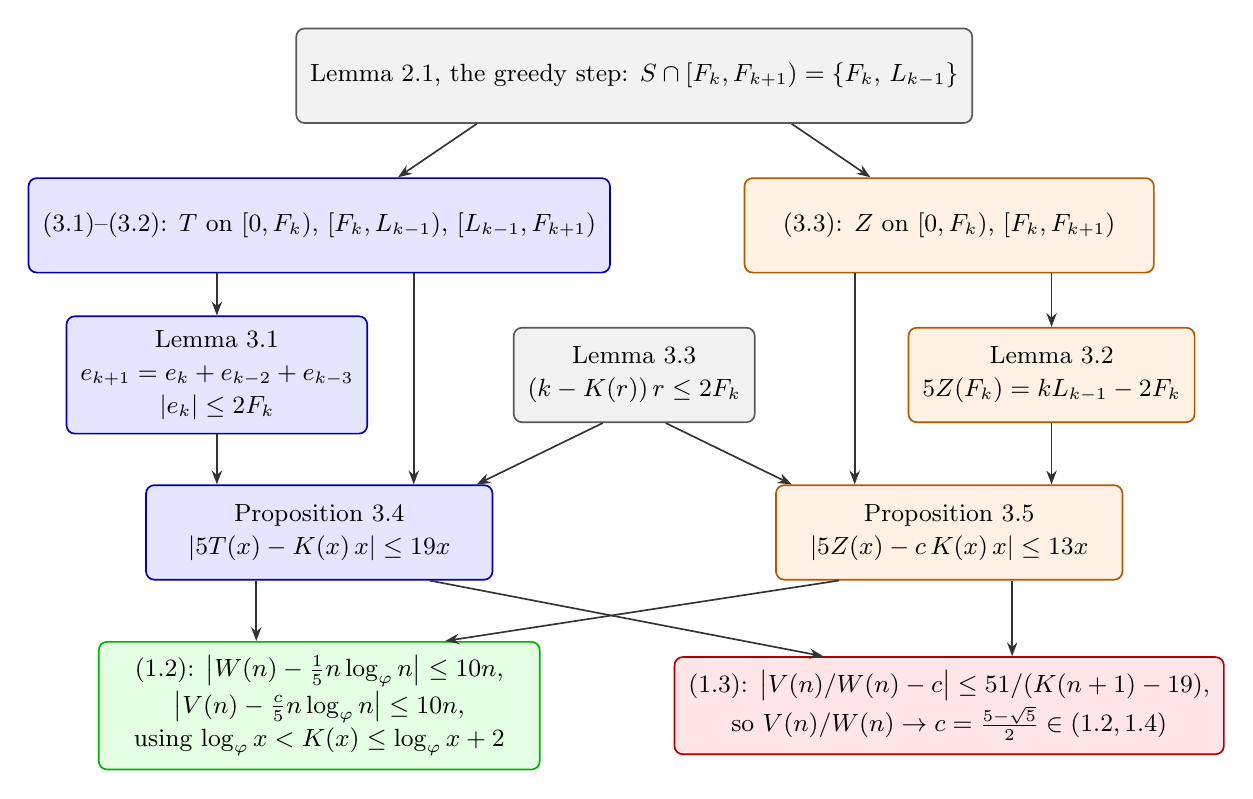
\begin{tikzpicture}[
  box/.style={draw=#1!70!black,fill=#1!10,rounded corners=3pt,line width=0.6pt,
              align=center,font=\small,inner sep=5pt,minimum height=12mm},
  box/.default=gray,
  arr/.style={-{Stealth[length=5pt]},line width=0.6pt,gray!40!black}]
  \node[box=gray,minimum width=7cm] (blk) at (0,0)
    {Lemma 2.1, the greedy step: $S\cap[F_k,F_{k+1})=\{F_k,\,L_{k-1}\}$};
  \node[box=blue,minimum width=5.2cm] (Trec) at (-4,-1.9)
    {(3.1)--(3.2): $T$ on $[0,F_k)$, $[F_k,L_{k-1})$, $[L_{k-1},F_{k+1})$};
  \node[box=orange,minimum width=5.2cm] (Zrec) at (4,-1.9)
    {(3.3): $Z$ on $[0,F_k)$, $[F_k,F_{k+1})$};
  \node[box=blue,minimum width=3.3cm] (ek) at (-5.3,-3.8)
    {Lemma 3.1\\[1pt] $e_{k+1}=e_k+e_{k-2}+e_{k-3}$\\[1pt] $|e_k|\le 2F_k$};
  \node[box=gray,minimum width=3.0cm] (gap) at (0,-3.8)
    {Lemma 3.3\\[1pt] $(k-K(r))\,r\le 2F_k$};
  \node[box=orange,minimum width=3.3cm] (zf) at (5.3,-3.8)
    {Lemma 3.2\\[1pt] $5Z(F_k)=kL_{k-1}-2F_k$};
  \node[box=blue,minimum width=4.4cm] (PT) at (-4,-5.8)
    {Proposition 3.4\\[1pt] $|5T(x)-K(x)\,x|\le19x$};
  \node[box=orange,minimum width=4.4cm] (PZ) at (4,-5.8)
    {Proposition 3.5\\[1pt] $|5Z(x)-c\,K(x)\,x|\le13x$};
  \node[box=green,minimum width=5.6cm] (asym) at (-4,-8.0)
    {(1.2): $\bigl|W(n)-\tfrac15 n\log_\varphi n\bigr|\le10n$,\\[1pt]
     $\bigl|V(n)-\tfrac c5 n\log_\varphi n\bigr|\le10n$,\\[1pt]
     using $\log_\varphi x<K(x)\le\log_\varphi x+2$};
  \node[box=red,minimum width=5.6cm] (rate) at (4,-8.0)
    {(1.3): $\bigl|V(n)/W(n)-c\bigr|\le 51/(K(n+1)-19)$,\\[1pt]
     so $V(n)/W(n)\to c=\tfrac{5-\sqrt5}2\in(1.2,1.4)$};
  % arrows
  \draw[arr] ([xshift=-2cm]blk.south) -- ([xshift=1cm]Trec.north);
  \draw[arr] ([xshift=2cm]blk.south) -- ([xshift=-1cm]Zrec.north);
  \draw[arr] (ek.north |- Trec.south) -- (ek.north);
  \draw[arr] (zf.north |- Zrec.south) -- (zf.north);
  \draw[arr] ([xshift=1.2cm]Trec.south) -- ([xshift=1.2cm]PT.north);
  \draw[arr] ([xshift=-1.2cm]Zrec.south) -- ([xshift=-1.2cm]PZ.north);
  \draw[arr] (ek.south) -- (ek.south |- PT.north);
  \draw[arr] (zf.south) -- (zf.south |- PZ.north);
  \draw[arr] ([xshift=-0.4cm]gap.south) -- ([xshift=2cm]PT.north);
  \draw[arr] ([xshift=0.4cm]gap.south) -- ([xshift=-2cm]PZ.north);
  \draw[arr] ([xshift=-0.8cm]PT.south) -- ([xshift=-0.8cm]PT.south |- asym.north);
  \draw[arr] ([xshift=0.8cm]PZ.south) -- ([xshift=0.8cm]PZ.south |- rate.north);
  \draw[arr] ([xshift=1.4cm]PT.south) -- ([xshift=-1.6cm]rate.north);
  \draw[arr] ([xshift=-1.4cm]PZ.south) -- ([xshift=1.6cm]asym.north);
\end{tikzpicture}
\end{document}
